%\chapter{MULTI-OBSERVATORY SPECTRAL ANALYSIS OF SUPERSOFT X-RAY SOURCES} \label{chap:multi-obs}
\chapter{\MakeUppercase{\ChapterTitleThree}} \label{chap:multi-obs}
    %\doublespacing
    \minitoc
    
    \newpage
    \begin{center}
    	%\emph{Abstract of chapter \ref{chap:multi-obs}}
    	\emph{Abstract}
    \end{center}
    
    In this chapter, we present a comprehensive study on the spectral characteristics and parameters of the supersoft X-ray source \source. We utilize a dataset comprising of six observations conducted by four different space observatories, namely ASCA, Chandra, XMM-Newton and NICER, spanning a time period of 25 years. Our objective is to identify a robust NLTE spectral model that can provide an acceptable fit to the continuum spectrum of \source, which had not been performed earlier as per current literature, thereby enhancing our understanding of its astrophysical nature. The study employs rigorous spectral modeling and comparative analysis to establish a framework for characterizing the continuum spectrum of \source. The study also discusses the analysis of the supersoft spectrum of \source, including the challenges in reproducing its spectra using NLTE model atmospheres. The best-fit model consists of a pure hydrogen NLTE model with effective gravity of 7, in conjunction with photoelectric absorption, ISM absorption and edge components. The effective temperature is found to be approximately of the order of $\sim 10^5$ K for all six observations, suggesting the presence of a hot accretion disk surrounding the white dwarf, which accretes matter from a companion main-sequence star. The study also analyzes the relative strengths of absorption edges in the spectrum and notes inconsistencies in the NICER observations. {The current work demonstrates that while the continuum spectrum of \source\ can be fitted satisfactorily, the same cannot be said to be the case for its high-resolution grating spectra. Therefore, it makes a case for the need to explore and develop methods that study such latest grating spectra, so as to obtain a more nuanced view of the astrophysics involving \source.}
    
    \newpage
    \section{Literature Review} \label{multi-obs:lit-rev}
    	Supersoft X-ray sources (SSS) represent an important class of celestial objects. They were initially recognized as a distinct class of intrinsically luminous X-ray sources by Trümper \textit{et al.} \cite{trumper1991x}, Greiner \textit{et al.} \cite{greiner1991rosat}, and Kahabka \textit{et al.} \cite{kahabka97}. These sources are classified based on their X-ray luminosities, which are typically around the Eddington limit ($\sim 10^{38}$ erg s$^{-1}$), indicating their exceptionally high brightness. However, their defining feature is their extremely soft X-ray spectra, with weak or negligible emission beyond $\sim 1$ keV and effective blackbody temperature no more than $\sim 100$ eV (or $\lesssim 1200$ kK) \cite{kahabka06}. The understanding of the spectral characteristics of SSS promises to pave the way for a deeper exploration of their role in the broader astrophysical landscape.
    	
    	SSS were initially observed by the Einstein Observatory during a soft X-ray survey of the Large Magellanic Cloud (LMC) by Long et al. in 1981 \cite{long81}. Over time, hundreds of objects exhibiting similar characteristics have been documented, many of which are considered candidates or confirmed members of this class. The catalog of SSS has expanded significantly, now encompassing sources not only within the LMC but also various other celestial bodies, including the Milky Way (MW), Small Magellanic Cloud (SMC), and Andromeda (M31) and numerous other galaxies \cite{kahabkatrumper1996,steinerdiaz1998,greiner2000,pietsch2003deep,di2003luminous,orio2010census,henze2010recent,sturm2012new,galiullin2021populations}.
    	
    	The relatively fewer detections of SSS within our galaxy, compared to other galaxies, may be attributed to significant interstellar extinction of soft X-rays. Situated at the edge of the MW and along its galactic plane, soft X-rays emitted by galactic SSS face considerable interstellar absorption. Suggestions have been made that SSS within the galactic plane must be within a distance of approximately 1 kpc to remain observable. Beyond this distance, interstellar absorption becomes sufficiently pronounced to render them undetectable \cite{van1992accreting}.
    	
    	The optical spectra of the SSS in the Magellanic Cloud galaxies exhibit similarities with those of low-mass X-ray binaries -- characterized by strong emission lines such as He II at 4686 \AA\ and hydrogen Balmer lines. Subsequent numerical calculations suggested that SSS could result from near-Eddington accretion onto neutron stars \cite{kylafis93}, although subsequent analyses favoured white dwarfs as the likely compact objects responsible for the emission of supersoft X-rays \cite{vandenHeuvel92}.
    	
    	Employing Stefan-Boltzmann's law with typical luminosity and effective temperature values for SSS, the estimated radius of the emitting object aligns with that of a white dwarf, supporting the hypothesis of accretion onto white dwarfs as the source of supersoft X-rays, akin to accreting neutron stars and black holes in classical X-ray binaries. Van den Heuvel proposed that white dwarfs with masses in the range $0.7–1.4\,M_\odot$ and mass accretion rates $\sim 1-5\times 10^{-7}\,M_\odot\text{ yr}^{-1}$ produce supersoft X-rays, assuming the mass-accretor as the white dwarf and the companion as a main-sequence or post-main-sequence star within specific mass ranges \cite{van1992accreting}. Studies by various groups have explored different types of nuclear burning due to mass accretion on white dwarfs, depending on the thermal history of the white dwarf and conditions required for nuclear ignition, typically involving critical envelope masses %$\Delta M_\text{crit}$
    sustaining high temperatures ($\sim 10^8$ K) and pressures ($\gtrsim 10^{18}-10^{20}$ g cm$^{-1}$ s$^{-2}$) for nuclear burning via the CNO cycle \cite{paczynski78,prialnik78,sion79,sienkiewicz80,nomoto82,fujimoto82a,fujimoto82b,iben82,prialnik95,macdonald83}. The steady state accretion rate, crucial for understanding the relationship between accretion and nuclear burning, has been investigated in early calculations \cite{paczynski80,iben82}, providing insights into the dynamics of hydrogen-rich matter accretion on white dwarfs. For a hydrogen-rich system, the steady state accretion rate was given to be \cite{hachisu2001}
		\begin{align}
			\dot{M}_\text{steady}\sim 3.7\times 10^{-7}\left( \dfrac{M_\text{WD}}{M_\odot}-0.4 \right)\,M_\odot\,\text{yr}^{-1} \label{eqn:steady-mass-accr}
		\end{align}
	
		The particular luminous galactic SSS known as MR Vel, and referred to as \source, was discovered by Motch \textit{et al.} \cite{motch1994} in the ROSAT Galactic Plane Survey (RGPS), which  is defined as the $|b|\leqslant 20\degree$ region of the ROSAT All Sky Survey. In the J2000 frame, the right ascension and declination of \source\ is 141.44042 and -47.96972 ($\alpha$=09 25 46.00, $\delta$=-47 58 17.4: as resolved by Simbad\footnote{\url{http://simbad.u-strasbg.fr/simbad/}}).
		
		\source\ was the brightest SSS candidate source in RGPS, with ROSAT PSPC hardness ratios of $HR1=0.96\pm 0.03$ and $HR2=-0.69\pm 0.03$. Fitting a blackbody to the ROSAT observations, a hydrogen column density in the range $n_H=(1.4-3.7)\times 10^{22}$ cm$^{-2}$ can be obtained. There is a considerable amount of uncertainty in current literature about its distance, with estimates ranging from 1 kpc to 10 kpc. Consulting Gaia Data Release 3\footnote{\url{https://www.cosmos.esa.int/web/gaia/data-release-3}}, one can find negligible parallax. This fact along with its high luminosity suggests that its distance is likely to be $>5$ kpc.
		
		Hartmann \textit{et al.} applied non-local thermodynamic equilibrium (NLTE) models, which included metal line opacities, to the spectrum extracted from the observations by BeppoSAX LECS of RX J0925 on January 25-26 1997 \cite{hartmann1999constraining}. They found that if a single model component is assumed for \source, a large discrepancy is observed between the model and data above 1.19 keV. The emission above $\sim 1.2$ kev (i.e. Ne IX edge) can be accounted for by adding another spectral model component, namely collisional ionization equilibrium.
		
		Higher resolution data obtained using the grating instruments on-board the Chandra and XMM-Newton observatories revealed complex structures in the spectra of \source. Such spectra show the presence of P Cygni profiles of Fe XVII and O VIII, which typically arise in a wind. Earlier, Bearda et al. (2002) and Motch et al. (2002) had come to the conclusion that the \source\ spectra, as observed by the Chandra HETGS and the XMM-Newton RGS, cannot be reproduced by LTE or NLTE model atmospheres \cite{beardaChandra2002AA,motchXmmNewton2002AA}, even though there is little clarity on the reason for this. Obtaining an acceptable fit for \source\ spectrum assumes crucial importance at this juncture. In the absence of a proper model describing the emission spectrum, it becomes impossible to calculate its parameters such as effective temperature and luminosity.
		
		In the present work, our primary objective was to identify a robust spectral model capable of providing an acceptable fit to the continuum spectrum of \source. To this end, we devised an approach wherein we analyse spectral data for \source\ obtained using multiple observatories. A motivation for harnessing such multi-observatory science data over an extended period was to mitigate potential biases associated with individual instruments and temporal variations in observational conditions, thereby enabling a systematic examination of the source's spectral characteristics, in an attempt to constrain the underlying physical processes driving the observed supersoft X-ray emission.
		
		The amalgamation of observations from diverse space observatories offered unique insights into the spectral evolution of the supersoft X-ray source over time, shedding light on its dynamic behavior and emission properties. Through rigorous spectral modeling and comparative analysis, we made an attempt to establish a robust framework for characterizing the continuum spectrum of the supersoft source, thereby enhancing our understanding of its astrophysical nature and evolutionary trends. A comprehensive investigation into recurrent SSS like \source\ is paramount due to the emerging recognition of SSS as progenitors of type Ia supernovae, which serve as crucial standard candles in cosmology. By delving deeper into the astrophysical mechanisms governing SSS, we can potentially enhance our ability to make precise predictions regarding the occurrence of type Ia supernovae and subsequently refine cosmological distance measurements.
    
    \begin{landscape}
    \section{Journal of Observations} \label{multi-obs:journal}
    	A summary of the observations used in this study, which included science data from Japan's ASCA \cite{ebisawaAsca2001ApJ}, NASA's Chandra \cite{beardaChandra2002AA}, ESA's XMM-Newton \cite{motchXmmNewton2002AA} and ISS' NICER \cite{orioNicer2022ApJ} observatories, is presented in table \ref{tab:obs-journal}.
    	
    	\renewcommand{\arraystretch}{2.2}
    	\begin{table}[!htb]
	    	\centering
	    	\caption{Journal of observations}
	    	\label{tab:obs-journal}
			\begin{tabular}{ccccccc}
				\hline
				\textbf{\begin{tabular}[c]{@{}c@{}}Observation\\ (Obs. ID)\end{tabular}} & \textbf{\begin{tabular}[c]{@{}c@{}}Date\\ (yyyy-mm-dd)\end{tabular}} & \textbf{Observatory} & \textbf{Instrument} & \textbf{MJD}$^\dagger$ & \textbf{\begin{tabular}[c]{@{}c@{}}Exposure$^\ddagger$\\ (ks)\end{tabular}} & \textbf{Region (keV)} \\
				\hline
				{43036000}   & {1994-12-22} & {ASCA} & {SIS1}          & {49708.56} & {20.58} & {0.20--1.00} \\
				{644}        & {2000-11-14} & {Chandra} & {ACIS}       & {51862.92} & {57.40} & {0.40--1.00} \\
				{0111150101} & {2000-12-16} & {XMM-Newton} & {EPIC-pn} & {51894.46} & {61.10} & {0.30--1.00} \\
				{2611020101} & {2019-05-18} & {NICER} & {XTI}          & {58621.90} & {2.53} & {0.40--1.00}  \\
				{2611020102} & {2019-05-19} & {NICER} & {XTI}          & {58622.03} & {8.57} & {0.45--1.00}  \\
				{2611020103} & {2019-05-19} & {NICER} & {XTI}          & {58623.00} & {9.91} & {0.45--1.00}  \\
				\hline
			\end{tabular}
			
			\begin{minipage}{16cm}
				\vspace{0.1cm}
				\small $^\dagger$Modified Julian Date
				
				\small $^\ddagger$From HEASARC archival query results
			\end{minipage}
		\end{table}
		\renewcommand{\arraystretch}{1.6}
	\end{landscape}
		
		During the course of our investigation of the continuum spectrum of \source, we leveraged a comprehensive dataset comprising six observations conducted by four distinct space observatories spanning the years 1994 to 2019. We extracted spectral data within the range 0.2 -- 1.0 keV from each observation in this dataset. This afforded us the opportunity to apply a consistent spectral analysis approach across a broad temporal range and disparate instrumentation platforms.
    
    \section{Data Reduction and Analysis} \label{multi-obs:red-analysis}
    	The raw data pertaining to all of the observations were downloaded using the online archival query interface at the \textit{High Energy Astrophysics Science Archive Research Center} (HEASARC)\footnote{\url{https://heasarc.gsfc.nasa.gov/db-perl/W3Browse/w3browse.pl}}. The data was reduced finally to \textit{Flexible Image Transport System} (FITS)\footnote{\url{https://fits.gsfc.nasa.gov/standard40/fits_standard40aa-le.pdf}} format using the software tools for the corresponding observatory with recommended settings in the relevant data analysis threads, wherever available. For the final analysis, a set of four files were generated for each of the observations. As a standard practice, these files were given the extensions as per a convention adopted by the authors as follows:
	    \begin{enumerate}
	    	\item Source spectrum, with file extension \texttt{.src}
	    	\item Background spectrum, with file extension \texttt{.bkg}
	    	\item Redistribution matrix file (RMF), with file extension \texttt{.rmf}
	    	\item Ancillary response file (ARF), with file extension \texttt{.arf}
	    \end{enumerate}
	    The above files were grouped using the FTOOLS task \texttt{grphha}\footnote{\url{https://heasarc.gsfc.nasa.gov/docs/heasarc/caldb/docs/memos/cal_sw_93_010/cal_sw_93_010.pdf}} to have an appropriate minimum number of counts per bin. The resulting spectrum sets were analysed using \textit{XSPEC} version 12.13.1.
    
    	\subsection{XMM-Newton EPIC-pn Data Reduction} \label{multi-obs:red-analysis:epic-pn}
    		The SSS \source\ was observed by all the instruments, viz. EPIC-MOS 1, EPIC-MOS 2, EPIC-pn and RGS, on-board ESA's XMM-Newton observatory for $\sim 52$ ks on 16 December 2000. Whereas, we had retrieved data from all the instruments, we decided to use only the EPIC-pn data. The reason for this being two-fold:
	    	\begin{enumerate}[i.]
	    		\item The spectral region of interest is of the lowest energies detectable by EPIC, and the pn detector has a comparatively higher sensitivity than the MOS detectors at lower energies \cite{stecchini2023revisiting,mateos2009statistical}.
	    		\item Currently, the high resolution grating spectra (such as those produced by the RGS) yield unacceptable fits to atmosphere models of SSS. Also, no atmosphere model has yet been able to reproduce all the details in such grating spectra \cite{ness2020complications}.
	    	\end{enumerate}
	    	As per recommendations by the XMM-Newton SOC, the data analysis was restricted to energies above 0.2 keV\footnote{\url{https://xmmweb.esac.esa.int/docs/documents/CAL-TN-0018.pdf}}. The data reduction procedures were performed using the \textit{XMM-Newton Science Analysis System} (SAS) version 21.0.0.
	    
	    	The Observation Data Files (ODF) were downloaded from HEASARC. In order to prepare the data for processing, we included the instrumental and calibration information by creating a Calibration Index File (CIF), which was up-to-date with the current calibration files (CCF)\footnote{\url{https://www.cosmos.esa.int/web/xmm-newton/current-calibration-files}}, and an extended ODF summary file. These were done by running the SAS tasks \texttt{cifbuild} and \texttt{odfingest} respectively. The ODFs were then reprocessed to generate the calibrated event files using the \texttt{epproc}, using the default parameters. The event file for EPIC-pn was filtered using the canned screening set of flags, and by setting \texttt{PATTERN==0} to select only single-pixel events in order to maximise energy calibration and resolution. The procedure described by Jethwa et al. (2015) \cite{jethwa2015pile} was used to check and find that the spectral distortion and flux loss both $<0.01\%$, which implied that the pile-up effects could be neglected.
	    	\begin{figure}[!htb]
		        \centering
		        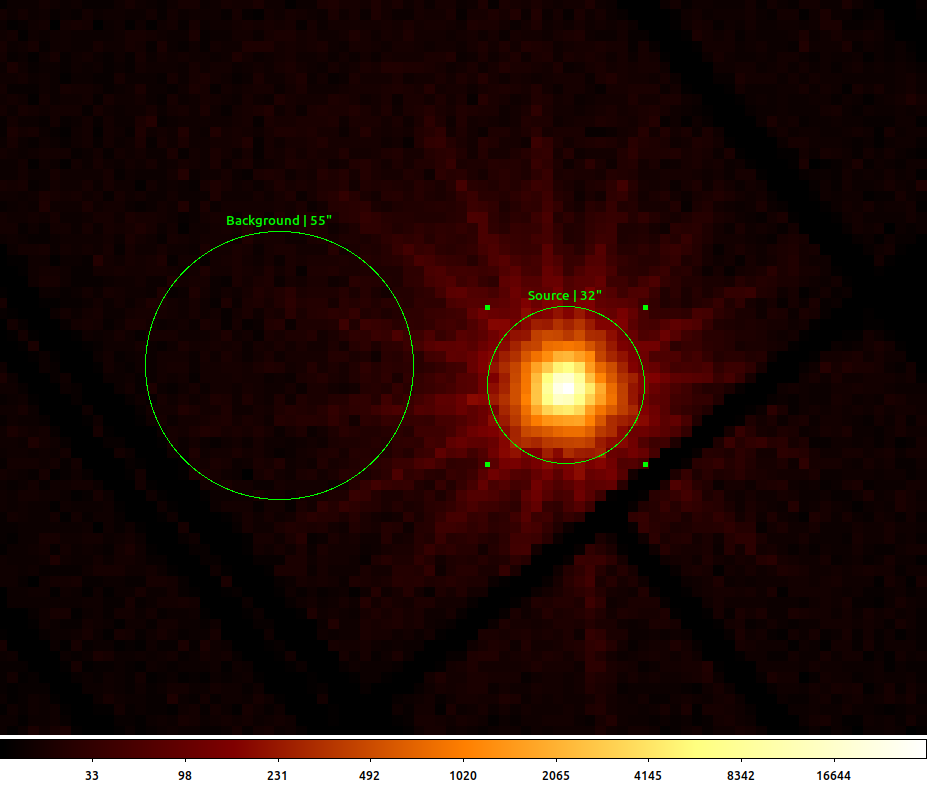
\includegraphics[width=0.8\textwidth]{images/rx-j0925-7-4758_0111150101_src-bkg.png}
		        \caption{Source and background extraction regions for the XMM-Newton observation of \source}
		        \label{fig:src-bkg:pn}
		    \end{figure}
		    
		    The source photons were idensified using DS9 and extracted from a circular region having a radius of 30" which is centred at the \source\ centroid position, encompassing about 85-90\% of XMM-Newton's telescope's on-axis PSF\footnote{\url{https://xmm-tools.cosmos.esa.int/external/xmm_user_support/documentation/uhb/onaxisxraypsf.html}}. For the background photons, first the SAS task \texttt{ebkgreg} was executed to obtain an optimum circular background extraction region of radius $\sim$55". The resulting source and background extraction regions are displayed in figure \ref{fig:src-bkg:pn}. The RMF and ARF were generated using the standard SAS tasks \texttt{rmfgen} and \texttt{arfgen}. The spectrum was finally binned to have a minimum of 10 counts/bin using the task \texttt{grphha} in order to make it ready for analysis using XSPEC.

    	
    	\subsection{ASCA SIS1 Data Reduction} \label{multi-obs:red-analysis:sis1}
    		\source\ was observed by the SIS1 instrument on-board Japan's ASCA observatory for a total duration of $\sim 21$ ks on 22 December 1994, with the purposes of characterization of its continuum spectral shape and the investigation of absorption edge features \cite{ebisawaAsca2001ApJ}. Because SIS1 has greater effective area for energies $<1.5$ keV\footnote{\url{https://heasarc.gsfc.nasa.gov/docs/asca/newsletters/sis_overview.html}}, the data analysis was restricted to an energy range of 0.2-1.0 keV. The procedures for the extraction of spectra were performed using \textit{XSELECT}\footnote{\url{https://heasarc.gsfc.nasa.gov/ftools/xselect/}} version 2.5, a multipurpose tool for filtering event files and generating images, spectra, and light curves made available as part of HEASoft.
    	
    		The event files were downloaded from HEASARC. They were loaded into XSELECT and the source and background spectra were extracted using a circular region of radius 127" and an annular region of radii 129" and 210" respectively, centred at \source\ centroid position. The RMF and ARF were generated using the FTOOL tasks \texttt{sisrmg}\footnote{\url{https://heasarc.gsfc.nasa.gov/lheasoft/ftools/fhelp/sisrmg.html}} and \texttt{ascaarf}\footnote{\url{https://heasarc.gsfc.nasa.gov/lheasoft/ftools/fhelp/ascaarf.html}} respectively. The spectrum set was grouped and binned to a minimum of 20 counts/bin using \texttt{grppha} so as to analyse using XSPEC.
    	
    	\subsection{Chandra ACIS Data Reduction} \label{multi-obs:red-analysis:acis}
    		\source\ was observed during 14 November 2000 for a duration of $\sim 57$ ks using the High-Energy Transmission Grating Spectrometer (HETGS) on-board NASA's Chandra X-ray Observatory \cite{beardaChandra2002AA}. The photons were detected with the ACIS-S CCD array at the focal plane. The data analysis was performed in the energy range 0.4--1.0 keV, with 0.4 keV being the lower limit of the HETGS+ACIS-S spectrometer combination. The extraction of the spectrum and response files was performed using \textit{CIAO} version 4.10 and the Chandra calibration database \textit{CALDB} version 4.7.7.
	    	\begin{figure}[!htb]
		        \centering
		        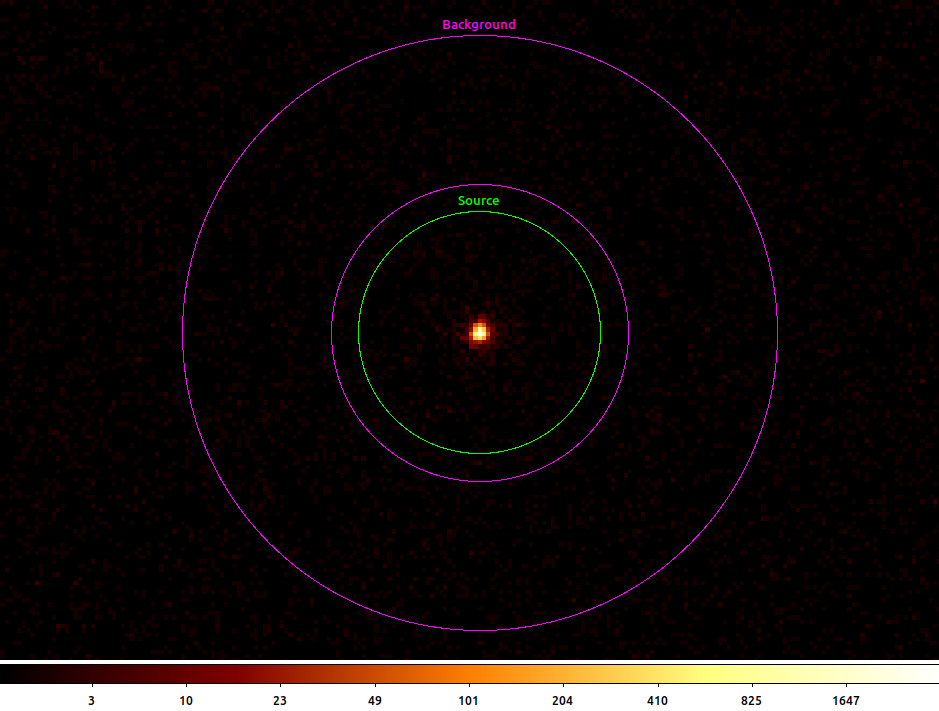
\includegraphics[width=0.8\textwidth]{images/rx-j0925-7-4758_644_src-bkg.png}
		        \caption{Source and background extraction regions for the Chandra observation of \source}
		        \label{fig:src-bkg:acis}
		    \end{figure}
	    	
	    	All the science data files were downloaded from HEASARC. DS9 was used to identify the source and background regions as being a circular region of radius 0.23' and an annular region of radii 0.28' and 0.57' respectively. The source and background spectra were extracted as FITS files using the task \texttt{specextract}\footnote{\url{https://cxc.cfa.harvard.edu/ciao/ahelp/specextract.html}} using standard parameters as per the data analysis threads for point-like sources\footnote{\url{https://cxc.cfa.harvard.edu/ciao/threads/pointlike/}}. The relevant RMF and ARF were generated using the \texttt{mkacisrmf}\footnote{\url{https://cxc.cfa.harvard.edu/ciao/ahelp/mkacisrmf.html}} and \texttt{mkarf}\footnote{\url{https://cxc.cfa.harvard.edu/ciao/ahelp/mkarf.html}} tasks respectively. The spectrum set was grouped and binned to have a minimum of 10 counts/bin using the task \texttt{grphha} for subsequent analysis using XSPEC.
    	
    	\subsection{NICER XTI Data Reduction} \label{multi-obs:red-analysis:xti}
    		\source\ was observed by the XTI instrument on-board the NICER observatory on the International Space Station (ISS) for a total duration of $\sim 21$ ks on three occasions during 18--19 May 2019. All data reduction commands for the science data were performed using NICER-specific tasks are made available with the latest versions of HEASoft\footnote{\url{https://heasarc.gsfc.nasa.gov/docs/software/heasoft/}}.
    	
	    	The XTI observation dataset and auxiliary files were downloaded from HEASARC. In order to prepare the data for processing, we set up the remote access of the HEASARC CALDB by following the recommended procedure\footnote{\url{https://heasarc.gsfc.nasa.gov/docs/heasarc/caldb/caldb_remote_access.html}}. The cleaned event files were extracted using the \texttt{nicerl2} command\footnote{\url{https://heasarc.gsfc.nasa.gov/lheasoft/ftools/headas/nicerl2.html}}. They were then loaded into XSELECT. This produces the source and background spectrum files in FITS format. The ARF and RMF were generated with the extracted source spectrum files using the \texttt{nicerarf}\footnote{\url{https://heasarc.gsfc.nasa.gov/lheasoft/ftools/headas/nicerarf.html}} and the \texttt{nicerrmf}\footnote{\url{https://heasarc.gsfc.nasa.gov/lheasoft/ftools/headas/nicerrmf.html}} commands respectively. The spectrum set was finally grouped and binned to a minimum of 10 counts/bin using \texttt{grphha} and made ready for analysis using XSPEC.
    	
    \section{Results} \label{multi-obs:results}
    	We present, in the following pages, a summary of the results of the analysis of the multi-observatory X-ray data for \source, including a comparison of the observed count rates, the stellar parameters calculated from the best-fit NLTE continuum models, the unfolded model spectra and the elemental absorption edges identified.
    	
    	
    	\subsection{Observed Count Rates} \label{multi-obs:results:count-rates}
    		In figures \ref{fig:all-counts:unnorm} and \ref{fig:all-counts:norm}, we present a comparison of count rates derived from the multi-observatory data listed in table \ref{tab:obs-journal}. Figure \ref{fig:all-counts:unnorm} serves to illustrate the variability of flux across different observation epochs, with count rates plotted on a logarithmic scale. This visualization provides insights into the temporal evolution of X-ray emission from \source.
    		
    		Concurrently, in figure \ref{fig:all-counts:norm}, the count rates are normalized to the range of 0 to 1 using \textit{min-max normalization}. This visualization accentuates the relative sensitivity of more recent observations to supersoft X-ray photons emitted by \source. The sub-plot shows that in recent observations the supersoft X-ray features are discernibly enhanced. This might be suggestive of improved observational capabilities or heightened sensitivity to the emitted X-ray flux.
    		
    		\newpage
    		\begin{figure}[h!]
				\centering				
				\subfloat[Using count rates \label{fig:all-counts:unnorm}]{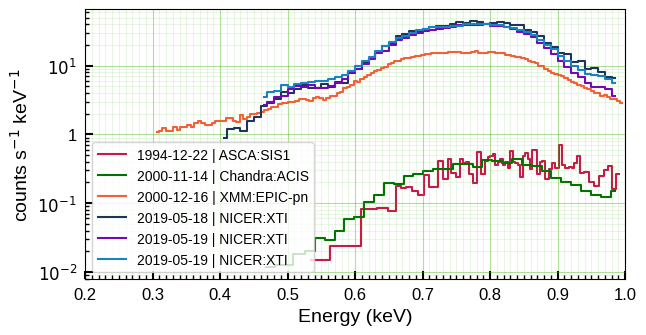
\includegraphics[width=0.9\textwidth]{images/ldata/mr-vel-counts_all-obs.png}}
				
				\subfloat[Using normalized count rates \label{fig:all-counts:norm}]{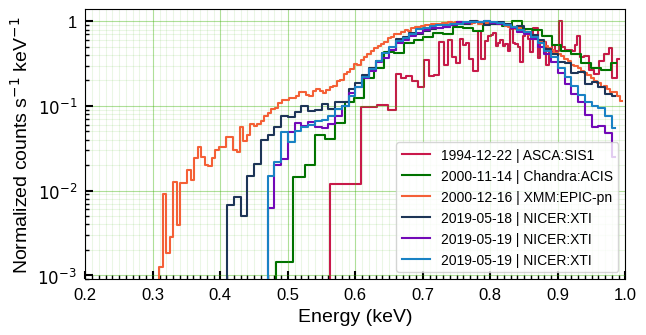
\includegraphics[width=0.9\textwidth]{images/ldata/mr-vel-normcounts_all-obs.png}}

				\caption{Comparison of flux from all observations}
		        \label{fig:all-counts}
			\end{figure}
			
%    		\begin{figure}[!htb]
%		        \centering
%		        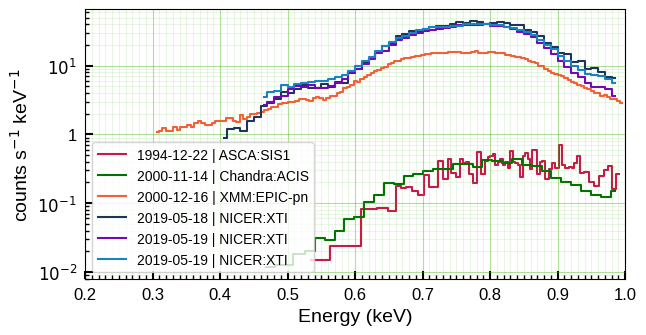
\includegraphics[width=0.8\textwidth]{images/ldata/mr-vel-counts_all-obs.png}
%		        \caption{Comparison of flux from all observations from their count rates plotted to scale}
%		        \label{fig:all-counts:unnorm}
%    		\end{figure}			
%			\begin{figure}
%				\centering
%		        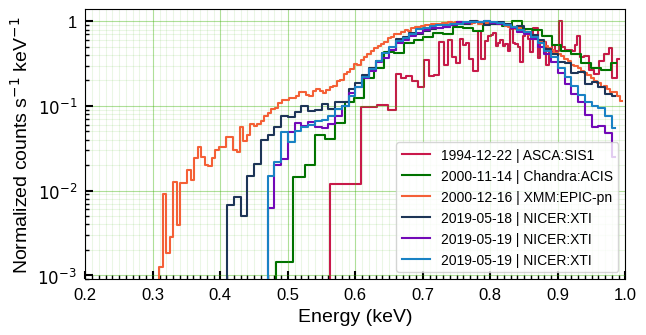
\includegraphics[width=0.8\textwidth]{images/ldata/mr-vel-normcounts_all-obs.png}
%		        \caption{Normalized count rates from all observations show varying responses to supersoft X-rays}
%		        \label{fig:all-counts:norm}
%		    \end{figure}
		    
		    Together, these visualizations offer a nuanced understanding of the flux variability and observational sensitivity trends exhibited by \source\ across different observation epochs, contributing to the broader understanding of its X-ray emission characteristics.
    	
    	\begin{landscape}
    	\subsection{NLTE Continuum Model} \label{multi-obs:results:nlte}
    		In table \ref{tab:res-fitting}, we present the luminosity, effective temperature and column density for \source\ which are derived after performing the fitting to the NLTE continuum model described in \S \ref{multi-obs:red-analysis} We also present the model fit statistics, namely the reduced $\chi^2$ values for each fit. It can be noticed that the same continuum model has been able to provide a good fit to all of the observations in our chosen dataset.
    		
    		\renewcommand{\arraystretch}{2.2}
    		\begin{table}[!htb]
		    	\centering
		    	\caption{Parameters of \source\ derived from continuum NLTE model from multi-observatory observations.}
		    	\label{tab:res-fitting}
		    	\begin{tabular}{ccccccc}
					\hline
					{\textbf{Observatory}} & {\textbf{Obs. ID}} & {$\boldsymbol{L_*}$ \textbf{(erg s$\boldsymbol{^{-1}}$)}} & {\textbf{$\boldsymbol{T_\text{eff}}$ (kK)}} & {\textbf{$\boldsymbol{n_H}$ ($\boldsymbol{\times 10^{22}}$ cm$\boldsymbol{^{-2}}$)}} & {$\boldsymbol{\chi^2}$/\textbf{d.o.f}} & {$\boldsymbol{\chi^2_\text{reduced}}$} \\
					\hline
					{ASCA} & {43036000} & {$2.07_{0.46}^{71.02}\times 10^{41}$} & {$100.2_{56.2}^{147.4}$} & {$0.13_{0.00}^{1.36}$} & {75.4/62} & {1.22} \\ %updated
					{Chandra} & {644} & {$4.38_{2.02}^{24.34}\times 10^{41}$} & {$96.3_{81.6}^{120.5}$} & {$1.25_{1.17}^{1.37}$} & {30.5/28} & {1.09} \\ %updated
					{XMM-Newton} & {0111150101} & {$2.19_{1.96}^{3.74}\times 10^{42}$} & {$91.7_{86.9}^{100.2}$} & {$1.17_{1.09}^{1.27}$} & {183.4/131} & {1.40} \\ %updated
					{NICER} & {2611020101} & {$8.40_{6.77}^{19.16}\times 10^{41}$} & {$100.8_{90.0}^{110.1}$} & {$1.22_{1.11}^{1.28}$} & {65.4/52} & {1.26} \\ %updated
					{NICER} & {2611020102} & {$1.68_{1.41}^{3.37}\times 10^{41}$} & {$107.9_{100.4}^{113.8}$} & {$0.46_{0.43}^{0.54}$} & {82.9/46} & {1.80} \\ %updated
					{NICER} & {2611020103} & {$4.41_{3.42}^{6.81}\times 10^{40}$} & {$106.9_{101.6}^{110.4}$} & {$0.36_{0.34}^{0.41}$} & {83.3/46} & {1.81} \\ %updated
					\hline
				\end{tabular}
			\end{table}
			\renewcommand{\arraystretch}{1.6}
			\end{landscape}
    	
    	\subsection{Unfolded Spectra from Best-fit Model} \label{multi-obs:results:unfolded}
    		In figures \ref{fig:all-uf:12-24} and \ref{fig:all-uf:24-36}, the unfolded spectrum, which is obtained after fitting the data to the best-fit model, is displayed. The observations reveal features which are indicative of the presence of elemental absorption edges.
    		
    		\begin{figure}[h!]
				\centering				
				\subfloat[Over the range 12 \AA - 24 \AA \label{fig:all-uf:12-24}]{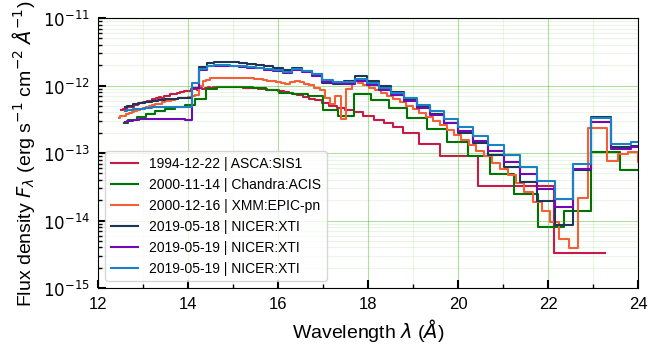
\includegraphics[width=0.9\textwidth]{images/eufspec/mr-vel-uf_all-obs_12-24.png}}
				
				\subfloat[Over the range 24 \AA - 36 \AA \label{fig:all-uf:24-36}]{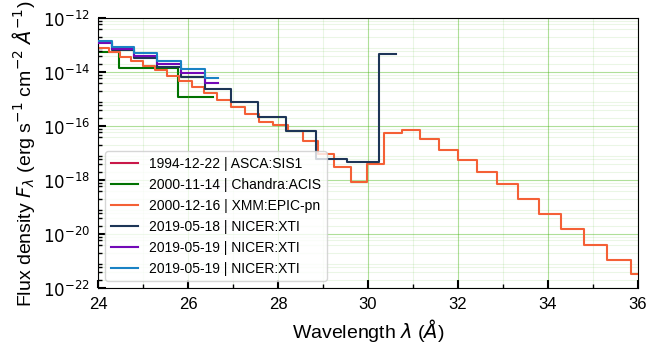
\includegraphics[width=0.9\textwidth]{images/eufspec/mr-vel-uf_all-obs_24-36.png}}

				\caption{Unfolded spectra after model fitting}
		        \label{fig:all-uf}
			\end{figure}
    		
%    		\begin{figure}[!htb]
%		        \centering
%		        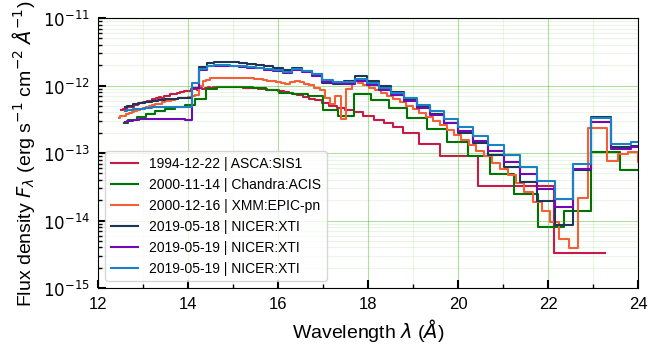
\includegraphics[width=0.9\textwidth]{images/eufspec/mr-vel-uf_all-obs_12-24.png}
%		        \caption{Unfolded spectra after model fitting in the range 12 \AA - 24 \AA}
%		        \label{fig:all-uf:12-24}
%		    \end{figure}
%
%		    \begin{figure}[!htb]
%		    	\centering
%		    	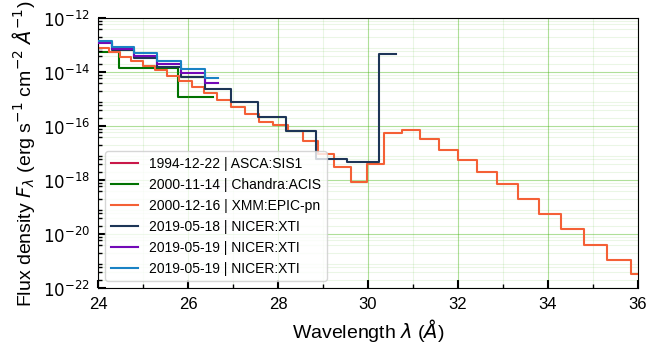
\includegraphics[width=0.9\textwidth]{images/eufspec/mr-vel-uf_all-obs_24-36.png}
%		    	\caption{Unfolded spectra after model fitting in the range 24 \AA - 36 \AA}
%		    	\label{fig:all-uf:24-36}
%		    \end{figure}
    	
    	\subsection{Luminosity versus Effective Temperature} \label{multi-obs:results:L-vs-Teff}
    		In figure \ref{fig:L-Teff}, we present a visualization of the calculated values of the luminosity $L_*$ and effective temperature $T_\text{eff}$ for \source\ using the best-fit model. One may note that the horizontal axis, containing the $T_\text{eff}$ data is plotted as increasing from right to left, \textit{\`{a} la} Hertzsprung-Russell diagram. This enables one to compare the overlap of the regions of uncertainty of these parameters as calculated using the data from multiple observatories.
    		
    		\begin{figure}[!thb]
		    	\centering
		    	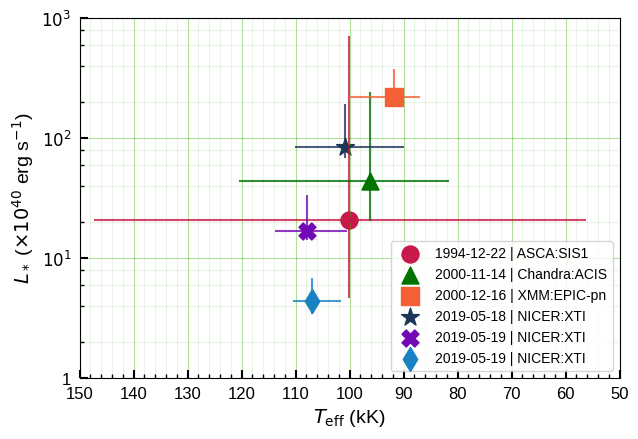
\includegraphics[width=0.9\textwidth]{images/L-Teff_all-obs.png}
		    	\caption{Uncertainties in $L_*$ and $T_\text{eff}$ calculations from multi-observatory observations of \source}
		    	\label{fig:L-Teff}
		    \end{figure}
    	
    	\subsection{Presence of Elemental Absorption Edges} \label{multi-obs:results:abs-edge}
    		During the preliminary fitting of the observations, the detection of residuals in absorption at energies of 0.402 keV, 0.532 keV, 0.708 keV and 0.867 keV suggested the presence of absorption edges. Consequently, by including relevant model components, four elemental absorption edges were detected from the best fitting model on all the observations. These absorption edges, belonging to N, O, Ne and Fe, are overlaid on the unfolded spectra and displayed in figure \ref{fig:all-uf:abs-edges}. The energies of the absorption edges were kept frozen during the fitting for all the observations.
    		
    		\begin{figure}[!htb]
		        \centering
		        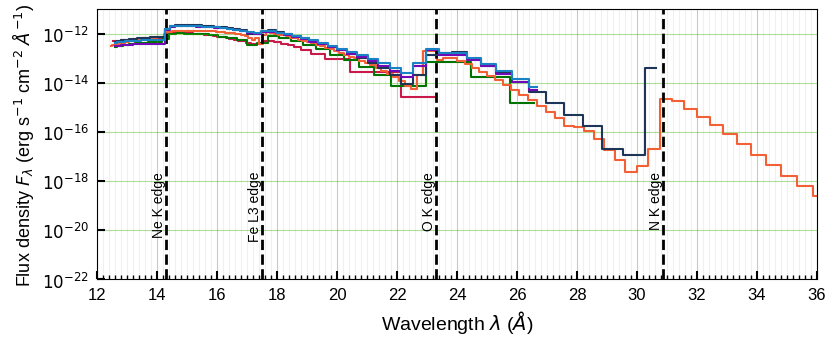
\includegraphics[width=\textwidth]{images/eufspec/mr-vel-uf-ang_abs-edge.png}
		        \caption{Unfolded spectra with overlaid elemental absorption edges}
		        \label{fig:all-uf:abs-edges}
		    \end{figure}
		    
		    Because the best-fitted spectrum obtained from the EPIC-pn instrument of XMM-Newton spans the widest range of wavelengths, known absorption edges \cite{bearden1967reevaluation,juett2006high} were identified in the vicinity of the absorption edges in figure \ref{fig:all-uf:abs-edges}. These are reported in table \ref{tab:abs-depth}. Then they were overlaid on the unfolded spectrum obtained from the EPIC-pn observation. The four absorption edges that could be identified are the $K$ edges of N, O and Ne and the $L_3$ edge of Fe at 30.873 \AA, 23.305 \AA, 14.302 \AA\ and 17.509 \AA\ respectively, as displayed in the sub-plots of figure \ref{fig:pn-uf:abs-edges}. Three among these four edges, namely the $K$ edges of O and Ne and the $L_3$ edge of Fe, were reported to be present in the spectrum of \source\ using the CLOUDY photoionization code by Prodhani and Baruah (2018) \cite{prodhani2018galactic}.
		    
		    \begin{figure}[h!]
				\centering				
				\subfloat[Ne K absorption edge at 14.302 \AA \label{fig:pn-uf:Ne-edges}]{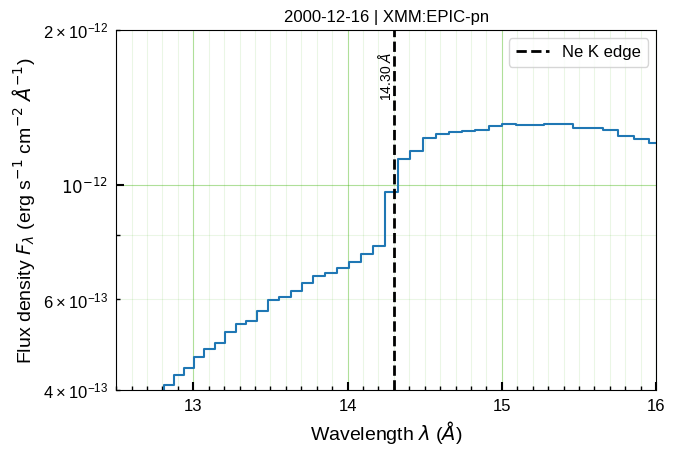
\includegraphics[width=0.5\textwidth]{images/eufspec/mr-vel-XMM-EPIC-pn-uf-Ne-edges.png}} %\hfill				
				\subfloat[Fe L$_3$ absorption edge at 17.509 \AA \label{fig:pn-uf:Fe-edges}]{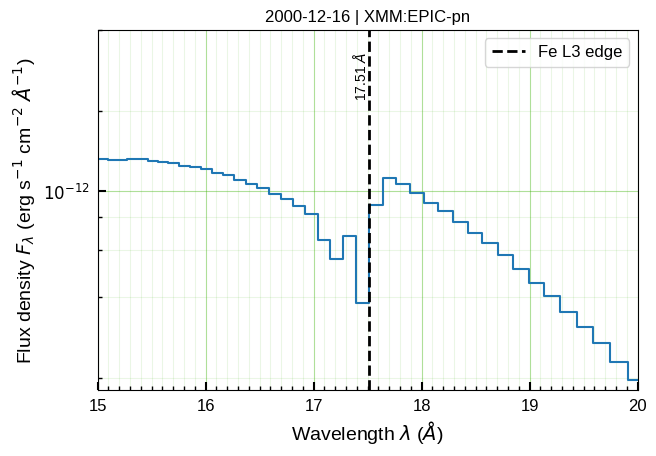
\includegraphics[width=0.5\textwidth]{images/eufspec/mr-vel-XMM-EPIC-pn-uf-Fe-edges.png}} %\hfill
				
				\subfloat[O K absorption edge at 23.305 \AA \label{fig:pn-uf:O-edges}]{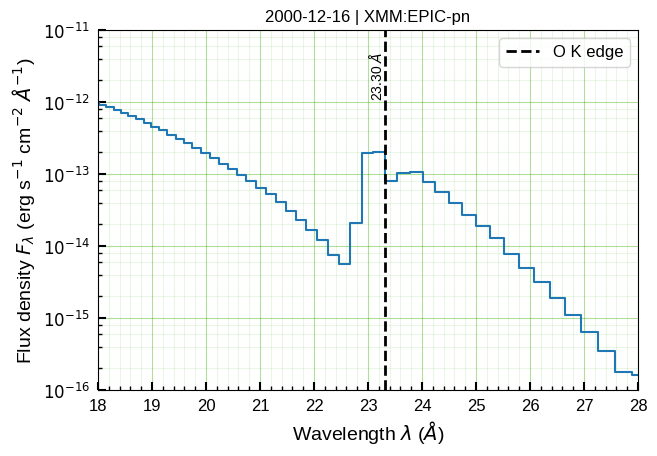
\includegraphics[width=0.5\textwidth]{images/eufspec/mr-vel-XMM-EPIC-pn-uf-O-edges.png}} %\hfill				
				\subfloat[N K absorption edge at 30.873 \AA \label{fig:pn-uf:N-edges}]{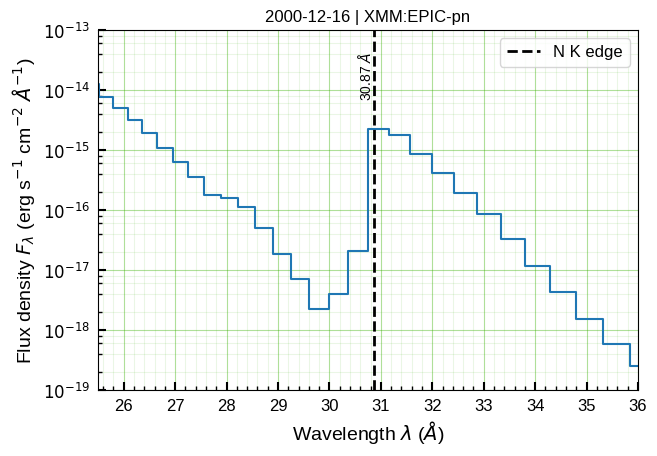
\includegraphics[width=0.5\textwidth]{images/eufspec/mr-vel-XMM-EPIC-pn-uf-N-edges.png}} %\hfill				
				\caption{Absorption edges for N, O, Ne and Fe overlaid on the unfolded spectrum for EPIC-pn observation}
		        \label{fig:pn-uf:abs-edges}
			\end{figure}
			
			\begin{landscape}
		    \renewcommand{\arraystretch}{2.2}
		    \begin{table}[!htb]
		    	\centering
		    	\caption{Absorption depth $D$ of \source\ derived from identified absorption edges of Ne, Fe, O and N.}
		    	\label{tab:abs-depth}
				\begin{tabular}{ccccccc}
					\hline
					\multirow{3}{*}{\textbf{Observatory}} & \multirow{3}{*}{\textbf{Obs. ID}} & \multicolumn{4}{c}{\textbf{Absorption Depth $\boldsymbol{D}$}} & \multirow{3}{*}{\textbf{Relative Depth}} \\ \cline{3-6} & & \textbf{Ne $\boldsymbol{K}$ edge} & \textbf{Fe $\boldsymbol{L_3}$ edge} & \textbf{O $\boldsymbol{K}$ edge} & \textbf{N $\boldsymbol{K}$ edge} \\ \cline{3-6} & & \textbf{14.302 \AA} & \textbf{17.509 \AA} & \textbf{23.305 \AA} & \textbf{30.873 \AA} \\
					\hline
					{ASCA} & {43036000} & {0.503} & {0.661} & {0.941} & {1.787} & {0.28 : 0.37 : 0.53 : 1.0} \\ %updated
					{Chandra} & {644} & {0.497} & {0.673} & {1.823} & {5.171} & {0.10 : 0.13 : 0.35 : 1.0} \\ %updated
					{XMM-Newton} & {0111150101} & {0.211} & {0.033} & {0.132} & {5.215} & {0.04 : 0.01 : 0.03 : 1.0} \\ %updated
					{NICER} & {2611020101} & {0.819} & {0.013} & {1.630} & {0.185} & {0.50 : 0.01 : 1.0 : 0.11} \\ %updated
					{NICER} & {2611020102} & {1.612} & {0.180} & {0.395} & {1.752} & {0.92 : 0.10 : 0.23 : 1.0} \\ %updated
					{NICER} & {2611020103} & {1.271} & {0.315} & {0.132} & {0.006} & {1.0 : 0.25 : 0.10 : 0.01} \\ %updated
					\hline
				\end{tabular}
			\end{table}
			\renewcommand{\arraystretch}{1.6}
		    \end{landscape}

    	
    \section{Discussion} \label{multi-obs:discussion}
    	As per current literature on spectral fitting of the SSS \source, Bearda et al. (2002) and Motch et al. (2002) had arrived at the conclusion that its spectra cannot be reproduced by NLTE model atmospheres \cite{beardaChandra2002AA,motchXmmNewton2002AA}. Earlier, Hartmann et al. (1999) had applied non-local thermodynamic equilibrium (NLTE) models, which included metal line opacities, to the spectrum extracted from the observations by BeppoSAX LECS of \source\ on 25--26 January 1997 \cite{hartmann1999constraining}, where the best fit was using a model consisting of two spectral components. But nevertheless, they obtained a reduced $\chi^2>2$. In the absence of a proper model describing the emission spectrum, it becomes impossible to
derive fundamental parameters such as temperature, neutral hydrogen column density and luminosity \cite{motchXmmNewton2002AA}. Hence, obtaining an acceptable fit for \source\ spectrum assumes crucial importance at this juncture.
    
    	\subsection{Best-fit Continuum Model} \label{multi-obs:discussion:cont-mod}
    		The model, chosen for fitting the data from six different observations, consists of a publicly available\footnote{\url{http://astro.uni-tuebingen.de/~rauch/TMAF/TMAF.html}} NLTE (non-local thermal equilibrium) table model component computed from a grid of stellar model atmosphere fluxes for source emission, a photoelectric absorption model component\footnote{\url{https://heasarc.gsfc.nasa.gov/xanadu/xspec/manual/XSmodelPhabs.html}}, a model component for absorption by inter-stellar medium\footnote{\url{https://heasarc.gsfc.nasa.gov/xanadu/xspec/manual/node255.html}} and four model components to account for the presence of absorption edges\footnote{\url{https://heasarc.gsfc.nasa.gov/xanadu/xspec/manual/node247.html}}.
    		
    		Figure \ref{fig:all-obs:resid-stats} presents the residual statistics from best-fit model to all observations. The values of the fit statistic used, i.e. the reduced $\chi^2$, were all within the acceptable range of $1<\chi^2_\text{reduced}<2$, which warrants a model to be considered a good fit for the observed data. An inspection of the distribution of the residual suggests an approximately normal distribution, which can be observed in the best-fit models for all the observations, further supporting the validity of the model fit. Such a distribution of the residuals is displayed in figure \ref{fig:pn:resid-hist} for the observations of the EPIC-pn data.
    		
    		\begin{figure}[h!]
				\centering				
				\subfloat[Residuals between data and best-fit model for EPIC-pn observations \label{fig:pn:resid}]{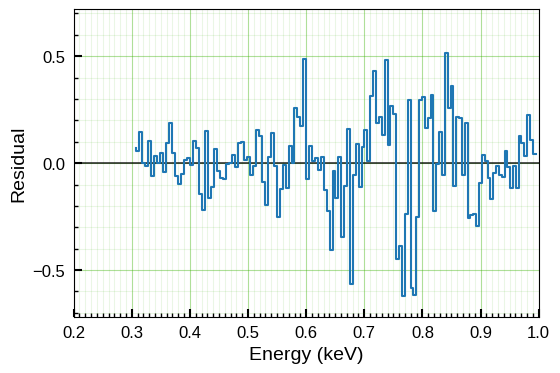
\includegraphics[width=0.48\textwidth]{images/resid/mr-vel-0111150101-pn_resid.png}} \hfill				
				\subfloat[Distribution of residuals from the best-fit model to EPIC-pn observations, along with the KDE function and fitted Gaussian \label{fig:pn:resid-hist}]{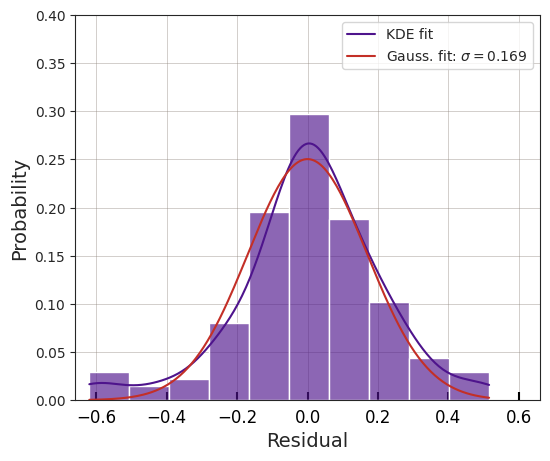
\includegraphics[width=0.48\textwidth]{images/resid/mr-vel-0111150101-pn_resid-hist.png}} %\hfill		
				\caption{Residual statistics from best-fit model to all observations}
		        \label{fig:all-obs:resid-stats}
			\end{figure}
			
			As it can be seen in figure \ref{fig:pn:resid-hist}, the kernel density estimate (KDE) function of the distribution closely approximates a normal distribution centred about zero (with zero indicating a perfect fit) and with a standard deviation of 0.169, thereby indicating that the observed count rate data can be considered to be random fluctuations which are normally distributed about the best-fit model. Therefore, the normal distribution of the residuals indicates that they are random and do not have a systematic bias (as is expected of a good fit), thereby further validating that the model fitting performed is satisfactory for all six cases of the observations.
			
			\begin{figure}[!htb]
		    	\centering
		    	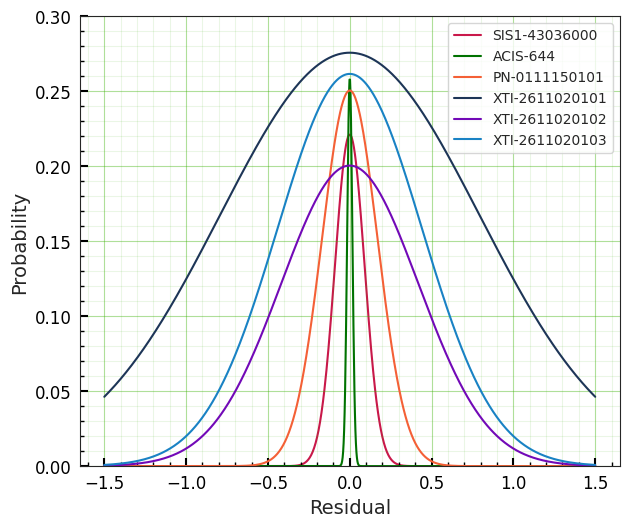
\includegraphics[width=0.8\textwidth]{images/resid/mr-vel-resid-gaussfit_all-obs.png}
		    	\caption{Gaussian approximations of the KDE functions for residual distributions of all observations}
		    	\label{fig:all-obs:resid-gaussfit}
		    \end{figure}
		    
		    In figure \ref{fig:all-obs:resid-gaussfit}, we find the Gaussian distribution fitted to all the observations. This figure shows that the quality of the fit is the best for the earlier Chandra, XMM-Newton and ASCA observations. For the recent NICER observations, the residuals show a wider spread spread about the perfect fit.
    	
    	\subsection{NLTE Pure H Model Atmosphere} \label{multi-obs:discussion:nlte-pureH}
    		In a classical stellar atmosphere, which is a plane-parallel, horizontally homogenous atmosphere in hydrostatic and radiative equilibrium, a non-LTE (or NLTE) description refers to a scenario where the energy levels of some selected species may be allowed to depart from their local thermodynamic equilibrium (LTE) values \cite{hubeny2014theory}.
    	
    		\subsubsection{Structural Equations}
    			Given below are the structural equations that are used to model an NLTE atmosphere.
    			
    			In its second-order form, the \textit{radiative transfer equation} is
    			\begin{align}
					\npdvt{2}{(f_\nu J_\nu)}{\tau_\nu}=J_\nu-S_\nu \label{eqn:rte-2nd-order}
				\end{align}
				where $J_\nu$ is the \textit{mean intensity} over all solid angles, $\tau_\nu$ the monochromatic \textit{optical depth}, $f_\nu$ the variable \textit{Eddington factor} and $S_\nu$ the \textit{source function}. The upper and lower boundary conditions on equation (\ref{eqn:rte-2nd-order}) are respectively
				\begin{align}
					&\left[ \pdvt{(f_\nu J_\nu)}{\tau_\nu} \right]_0=g_\nu J_\nu(0)-H_\nu^\text{ext} \label{eqn:rte-upper-bc} \\
					&\left[ \pdvt{(f_\nu J_\nu)}{\tau_\nu} \right]_{\tau_\text{max}}=H_\nu^+-\dfrac{1}{2}J_\nu \label{eqn:rte-lower-bc}
				\end{align}
				where $g_\nu$ is the \textit{surface Eddington factor}, $H_\nu^\text{ext}$, $H_\nu^+$ being the \textit{first angular moment} of specific intensity taken at the respective upper and lower boundaries of the current stellar atmospheric layer.
				
				The \textit{hydrostatic equilibrium equation} is re-cast as
				\begin{align}
					\dvt{P_\text{gas}}{m}=g-\dfrac{4\pi}{c}\integ{0}{\infty}{\dvt{K_\nu}{m}}{\nu}=g-\dfrac{4\pi}{c}\integ{0}{\infty}{\dfrac{\chi_\nu}{\rho}H_\nu}{\nu} \label{eqn:hyd-equil}
				\end{align}
				where $K_\nu$ is the \textit{second angular moment} of specific intensity, $\chi_\nu$ is the \textit{absorption coefficient} and $m$ is the \textit{Lagrangian mass}. In equation (\ref{eqn:hyd-equil}), the total pressure is composed of three parts: the \textit{gas pressure} $P_\text{gas}$, the \textit{radiation pressure} represented by the integrals on the right-hand side and the \textit{microturbulent pressure} $P_\text{turb}$ being ignored.
				
				The \textit{radiative equilibrium equation} is an expression of the conservation of total radiant flux. It may be written in an \textit{integral form} -- more accurate at upper atmospheric layer, or in a \textit{differential form} -- more accurate in deeper layers. To improve the accuracy, numerical algorithms implement a linear combination of both form as
				\begin{align}
					\alpha&\left[ \integ{0}{\infty}{(\kappa_\nu J_\nu-\eta_\nu)}{\nu} \right] \nonumber\\
						&+\beta\left[ \integ{0}{\infty}{\dvt{(f_\nu J_\nu)}{\tau_\nu}}{\nu}-\dfrac{\sigma_R}{4\pi}T_\text{eff}^4 \right]=0 \label{eqn:rad-equil}
				\end{align}
				where $\sigma_R$ is the Stefan-Boltzmann constant, $\kappa_\nu$, $\eta_\nu$ are the thermal absorption and emission coefficients respectively. In equation (\ref{eqn:rad-equil}) above, the term within the first pair of brackets contains the integral form and that within the second pair contains the differential form. The empirical coefficients $\alpha$, $\beta$ enable a transition from upper layers ($\alpha\rightarrow 1$, $\beta\rightarrow 0$) to lower layers ($\alpha\rightarrow 0$, $\beta\rightarrow 1$) -- such a transition is taken to be around the depth where the Rosseland mean optical depth is $\sim 1$.
				
				The \textit{kinetic equilibrium equations} (or \textit{rate equations}) are written for each chemical species, after having first selected those species which are to be considered to deviate from LTE. For any species, these equations may be represented by a matrix equation as
				\begin{align}
					\vsmat{A}\cdot\vsvec{n}=\vsvec{b} \label{eqn:kin-equil}
				\end{align}
				where the elements of the \textit{rate matrix} $\vsmat{A}$ are given as
				\begin{align*}
					\vmelem{A}{i}{j}&=\sum_{j\neq i}{(R_{ij}+C_{ij})} \\
					\vmelem{A}{i}{j}&=-(R_{ji}+C_{ji}),\text{ for }j\neq i\text{ and }i\neq k \\
					\vmelem{A}{k}{j}&=1+S_j
				\end{align*}
				with $k$ being the index of the \textit{characteristic level} and $R_{ij}$, $C_{ij}$ the radiative and collisional rates respectively between transition levels $i$ and $j$. It must be noted that $R_{ij}$'s implicitly involve the \textit{Saha-Boltzmann factor} $\Phi_i(T)$ which comes into play for \textit{bound-free transitions}, i.e. absorption edges
				\begin{align}
					\Phi_i(T)=\dfrac{g_i}{2g_1^+}\left( \dfrac{h^2}{2\pi m_e kT} \right)^{3/2}e^{(E_I-E_i)/kT} \label{eqn:saha-boltz-factor}
				\end{align}
				where $E_I$ is the ionization potential of the ion to which level $i$ belongs, $E_i$ the excitation energy of level $i$ and $g_1^+$ the statistical weight of the ground state of the next ion and $m_e$ the electronic mass. In equation (\ref{eqn:kin-equil}), $\vsvec{n}$ is the vector of populations of levels and the vector $\vsvec{b}$ has a single non-zero element corresponding to the characteristic level $k$ as
				\begin{align*}
					\vvelem{b}{i}=(N-n_e)\alpha_I\delta_{ki}
				\end{align*}
				where $N$ is the net populations of all levels, $n_e$ the number density of electrons and $\alpha_I$ the fractional abundance of the species $I$.
				
				The overall electrical neutrality of the medium is expressed by the \textit{charge conservation equation} as
				\begin{align}
					\sum_i{n_iZ_i}-n_e=0 \label{eqn:ch-cons}
				\end{align}
				where $Z_i$ is the charge associated with level $i$.
				
				The \textit{mass density}, which is related to the atomic level populations, can be expressed as
				\begin{align}
					\rho=(N-n_e)\mu m_H \label{eqn:mass-dens}
				\end{align}
				where $\mu$ is the mean molecular weight and $m_H$ is the mass of the H atom. A quantity known as the \textit{fictitious massive particle density} is defined as
				\begin{align}
					n_m\equiv(N-n_e)\mu \label{eqn:fict-mass-dens}
				\end{align}
				which then enables the mass density to be simply written as $\rho=n_m m_H$.
				
				The absorption coefficient included in equation (\ref{eqn:hyd-equil}) is written as the combination
				\begin{align}
					\chi_\nu=\kappa_\nu+\kappa_\nu^\text{sc} \label{eqn:abs-coeff}
				\end{align}
				where $\kappa_\nu$ is also known as the \textit{extinction coefficient} and $\kappa_\nu^\text{sc}$ the \textit{scattering coefficient}. The extinction coefficient is given as
				\begin{align}
					\kappa_\nu=\sum_{i}&\sum_{j>i}{[n_i-n_jG_{ij}(\nu)]\sigma_{ij}(\nu)} \nonumber\\
									&+\sum_{l}{n_en_l\sigma_{ll}(\nu,T)\left( 1-e^{-h\nu/kT} \right)}+\kappa_\nu^\text{addl} \label{eqn:ext-abs-coeff}
				\end{align}
				where the first term represents the contribution from \textit{bound-bound transitions} (i.e. absorption lines), the second represents that from \textit{bound-free transitions} (i.e. absorption edges) and the last term lumps together any additional opacity not written as detailed transitions. Here $G_{ij}=\frac{w_ig_i}{w_jg_j}$, with $g_i,g_j$ and $w_i,w_j$ being the respective degeneracies and statistical weights of levels $i$ and $j$ respectively. Also $\sigma_{ij}$ is the opacity of the transition between levels $i$ and $j$.
				
				The scattering coefficient in equation (\ref{eqn:abs-coeff}) is given as
				\begin{align}
					\kappa_\nu^\text{sc}=n_e\sigma_e + \sum_i{n_{\text{Ray},i}\sigma_{\text{Ray},i}} \label{eqn:sca-abs-coeff}
				\end{align}
				where $\sigma_e$, $\sigma_{\text{Ray},i}$ are the Thomson and Rayleigh scattering cross-sections respectively. For pure-hydrogen atmospheres with high temperatures, the Rayleigh scattering is negligible because the hydrogen atoms are expected to be fully ionized.
				
				In a similar manner, the \textit{total emission coefficient} is also expressed as a sum of thermal and scattering contributions as
				\begin{align}
					\eta_\nu^\text{total}=\eta_\nu+\eta_\nu^\text{sc} \label{eqn:em-coeff}
				\end{align}
				where
				\begin{align}
					\eta_\nu=\left(\dfrac{2h\nu^3}{c^2}\right)&\left[ \sum_{i}\sum_{j>i}{n_jG_{ij}(\nu)\sigma_{ij}(\nu)} \right. \nonumber\\
									&\left.+\sum_{l}{n_en_l\sigma_{ll}(\nu,T)e^{-h\nu/kT}}\right]+\eta_\nu^\text{addl} \label{eqn:ext-em-coeff}
				\end{align}
				in which, again, any additional emissivity is lumped together and given using the Planck function as $\eta_\nu^\text{addl}=\kappa_\nu^\text{addl}B_\nu$.
				
				Finally, taking into account the \textit{convective flux} $F_\text{conv}$ (if any) within the differential form of the radiative equilibrium equation (\ref{eqn:rad-equil}) as
				\begin{align}
					\integ{0}{\infty}{\dvt{(f_\nu J_\nu)}{\tau_\nu}}{\nu}+\dfrac{F_\text{conv}}{4\pi}=\dfrac{\sigma_R}{4\pi}T_\text{eff}^4 \label{eqn:rad-equil-2}
				\end{align}
				Differentiating equation (\ref{eqn:rad-equil-2}) with respect to the Lagrangian mass $m$ finally gives the \textit{radiative+convective equilibrium equation} as
				\begin{align}
					\integ{0}{\infty}{(\kappa_\nu J_\nu-\eta_\nu)}{\nu}+\dfrac{\rho}{4\pi}\dvt{F_\text{conv}}{m}=0 \label{eqn:rad-conv-equil}
				\end{align}
    		
    		\subsubsection{Numerical Solution using ALI}
    			Accelerated lambda iteration (ALI) is a technique used to numerically solve the radiative transfer problem, particularly in the context of stellar atmosphere modeling \cite{hubeny2003accelerated}. It accelerates the computational process by introducing a correction term that takes into account the influence of previous iterations. A simplified procedural overview of this scheme is as follows:
				\begin{enumerate}
					\item \textit{Initial guess}: Start with an initial guess for the specific intensity of radiation at different frequencies within the atmosphere. \label{step:ali-init-guess}
					\item \textit{Lambda iteration}: Calculate how the radiation interacts with the atmosphere using the current guess for intensity, considering the absorption and emission by the species in the atmosphere. \label{step:ali-lmda-itr}
					\item \textit{Correction term}: Instead of simply accepting the result from step \ref{step:ali-lmda-itr}, ALI calculates a correction term based on the difference between the current guess and the result. \label{step:ali-corr-term}
					\item \textit{Update guess}: Add this correction term to the initial guess to obtain a new estimate for the intensity. \label{step:ali-update-guess}
					\item \textit{Iterate}: Repeat steps \ref{step:ali-lmda-itr}--\ref{step:ali-update-guess} until the solution converges, meaning the intensity values no longer change significantly between iterations. \label{step:ali-iterate}
				\end{enumerate}
				
				In order to numerically solve the structural equations for NLTE, they are first discretized over all three continuous variables: optical depth $\tau$, frequency $\nu$ and angle $\theta$. These discretized structural equations, together with a number of auxiliary relations, form a system of highly coupled, non-linear equations. Then the \textit{complete linearization scheme} \cite{auer1970non} is used to treat all equations on the same footing, thus solving all structural equations simultaneously. The T\"{u}bingen NLTE Model Atmosphere Package (TMAP)\footnote{\url{http://astro.uni-tuebingen.de/~rauch/TMAP/TMAP.html}} code uses ALI to calculate the stellar atmosphere by taking into account metal line-blanketing. With an extended grid of such atmospheres of pure-hydrogen models, synthetic spectral were calculated and these are eventually used as table models in XSPEC in the present work to simulate the source emission.
    	
    	\subsection{Inferences from Results} \label{multi-obs:discussion:inference}
    		Here we are trying to understand the supersoft spectrum of \source, across observations from 1994 to 2019. The idea is to develop a robust model that explains its supersoft spectrum over different time scales and different observing instruments. The best-fit model consists of XSPEC model components which consider various factors affecting the observed spectrum:
		    \begin{enumerate}[a)]
		   		\item \texttt{atable\{}pure-H NLTE with $\log{g}=7$\texttt{\}}: for the actual radiation emitted by \source
		   		\item \texttt{edge}: for specific wavelengths where bound-free absorption is particularly strong, leading to absorption edges
		   		\item \texttt{phabs}: for describing the photoelectric absorption at the source itself.
		   		\item \texttt{ismabs}: for describing how light interacts with the intervening inter-stellar medium before reaching us
		   	\end{enumerate}
		   	
		   	Initially, a simple blackbody model failed to fit the spectrum. Blackbodies emit a characteristic spectrum based on temperature, and it seems this doesn't accurately represent the complex emission from \source. Then the supersoft X-ray emission of \source\ was modelled using an NLTE stellar atmosphere model \cite{werner1999classical}. Some of these are made available as tables in appropriate FITS format to be used with the XSPEC table model component \texttt{atable} \cite{rauch2003grid,rauch2010nlte}. These models, which are essentially pre-calculated grids, vary from one another in terms of the elemental abundances, the effective temperature $T_\text{eff}$ and the effective gravity $\log{g}$ (where the gravitational acceleration $g$ is expressed in cgs units). Choosing a particular FITS file fixed the specific elemental abundance and effective gravity. Then the fitting of the model to the data is performed by using the effective temperature $T_\text{eff}$ and the redshift $z$ as parameters.
    
		    During the analysis of the spectra from all six observations of \source, we found that only an NLTE model with a pure hydrogen atmosphere for which $\log{g}=7$ was able to provide a common model continuum spectrum that gave acceptable fit quality for all six observations. This model\footnote{\url{http://astro.uni-tuebingen.de/~rauch/TMAF/flux_H.html}}, developed and made publicly available by Rauch et al., has, as the core of its computational framework, the detailed representation of hydrogen atoms within stellar atmospheres. Using the TMAP,  plane-parallel, static, pure-hydrogen models were calculated, employing several simplifying assumptions to create a tractable model of the stellar atmosphere. Here, hydrogen is represented as a model atom, focussing on energy levels up to $n=14$ under NLTE conditions, neglecting the rapid depopulation of higher levels due to a compact star's strong gravity. Certain complexities like the exact treatment of light absorption are approximated for efficiency. Finally, the model only extends to a specific optical depths of
		    $$\log{\tau}=-8\dots+4$$
		    within the atmosphere where light can travel freely, and utilizes increased detail for calculations in specific wavelength range to ensure accuracy in that region. For the synthetic spectra, the line-broadening tables of Lemke (1997) were used \cite{lemke1997extended}.
		    
		    As it can be seen from table \ref{tab:res-fitting} and figure \ref{fig:L-Teff}, the effective temperature is obtained to be $\sim 10^5$ K for all six observations and luminosity is computed to be of the order of $10^{41}$ erg s$^{-1}$, which is about 3 orders of magnitude higher that what had been reported earlier \cite{hartmann1999constraining}. Such order of magnitude of $T_\text{eff}$ is also observed recently in similar fitting of CAL 83 spectrum using a pure-hydrogen NLTE model \cite{stecchini2023revisiting}. The high values of $T_\text{eff}$ and $L_*$ from a good fit using a pure-hydrogen model seem counterintuitive for an SSS, which is typically a white dwarf accreting from a companion star. This is because white dwarfs are usually much cooler, and the accreted material might not be pure hydrogen.
    
    		However, we need to take into account the currently accepted model for SSS which is the steady nuclear burning on the surface of a white dwarf. It is likely that the companion star to \source\ is a main-sequence star, thereby hydrogen-rich. Consequently, it is possible that only hydrogen-rich matter is able to accrete around the white dwarf. This matter, upon reaching the surface of the white dwarf, owing to its large gravity, undergoes steady nuclear burning. This may explain the success of the pure-hydrogen NLTE model in fitting its spectrum. It must be borne in mind that the high $T_\text{eff}$ likely characterizes the hot accretion disk surrounding the white dwarf, and not the white dwarf itself. Friction and compression may cause the accreting matter to attain the temperatures required to undergo steady nuclear burning.
    		
    		There are a couple of limitations to drawing such an inference regarding \source:
		    \begin{enumerate}[i.]
		    	\item The NLTE model assumes a static source, which might not be entirely accurate for a dynamic system like an accretion disk.
		    	\item The model assumes a pure-hydrogen composition, which might be a simplification of the actual accreting material.
		    \end{enumerate}
		    
		    Future modeling could explore relaxing some assumptions, such as including additional elements or allowing for a dynamic disk structure. One way to do so could be by utilising the high-resolution grating spectra from observatories, such as the reflection grating spectrometer (RGS) on-board XMM-Newton, to study the absorption line profiles observed in the spectrum of \source\ and analyzing the corresponding transitions can provide valuable insights into the dynamics of the accreting material.
		    
		    \begin{figure}[!htb]
		    	\centering
		    	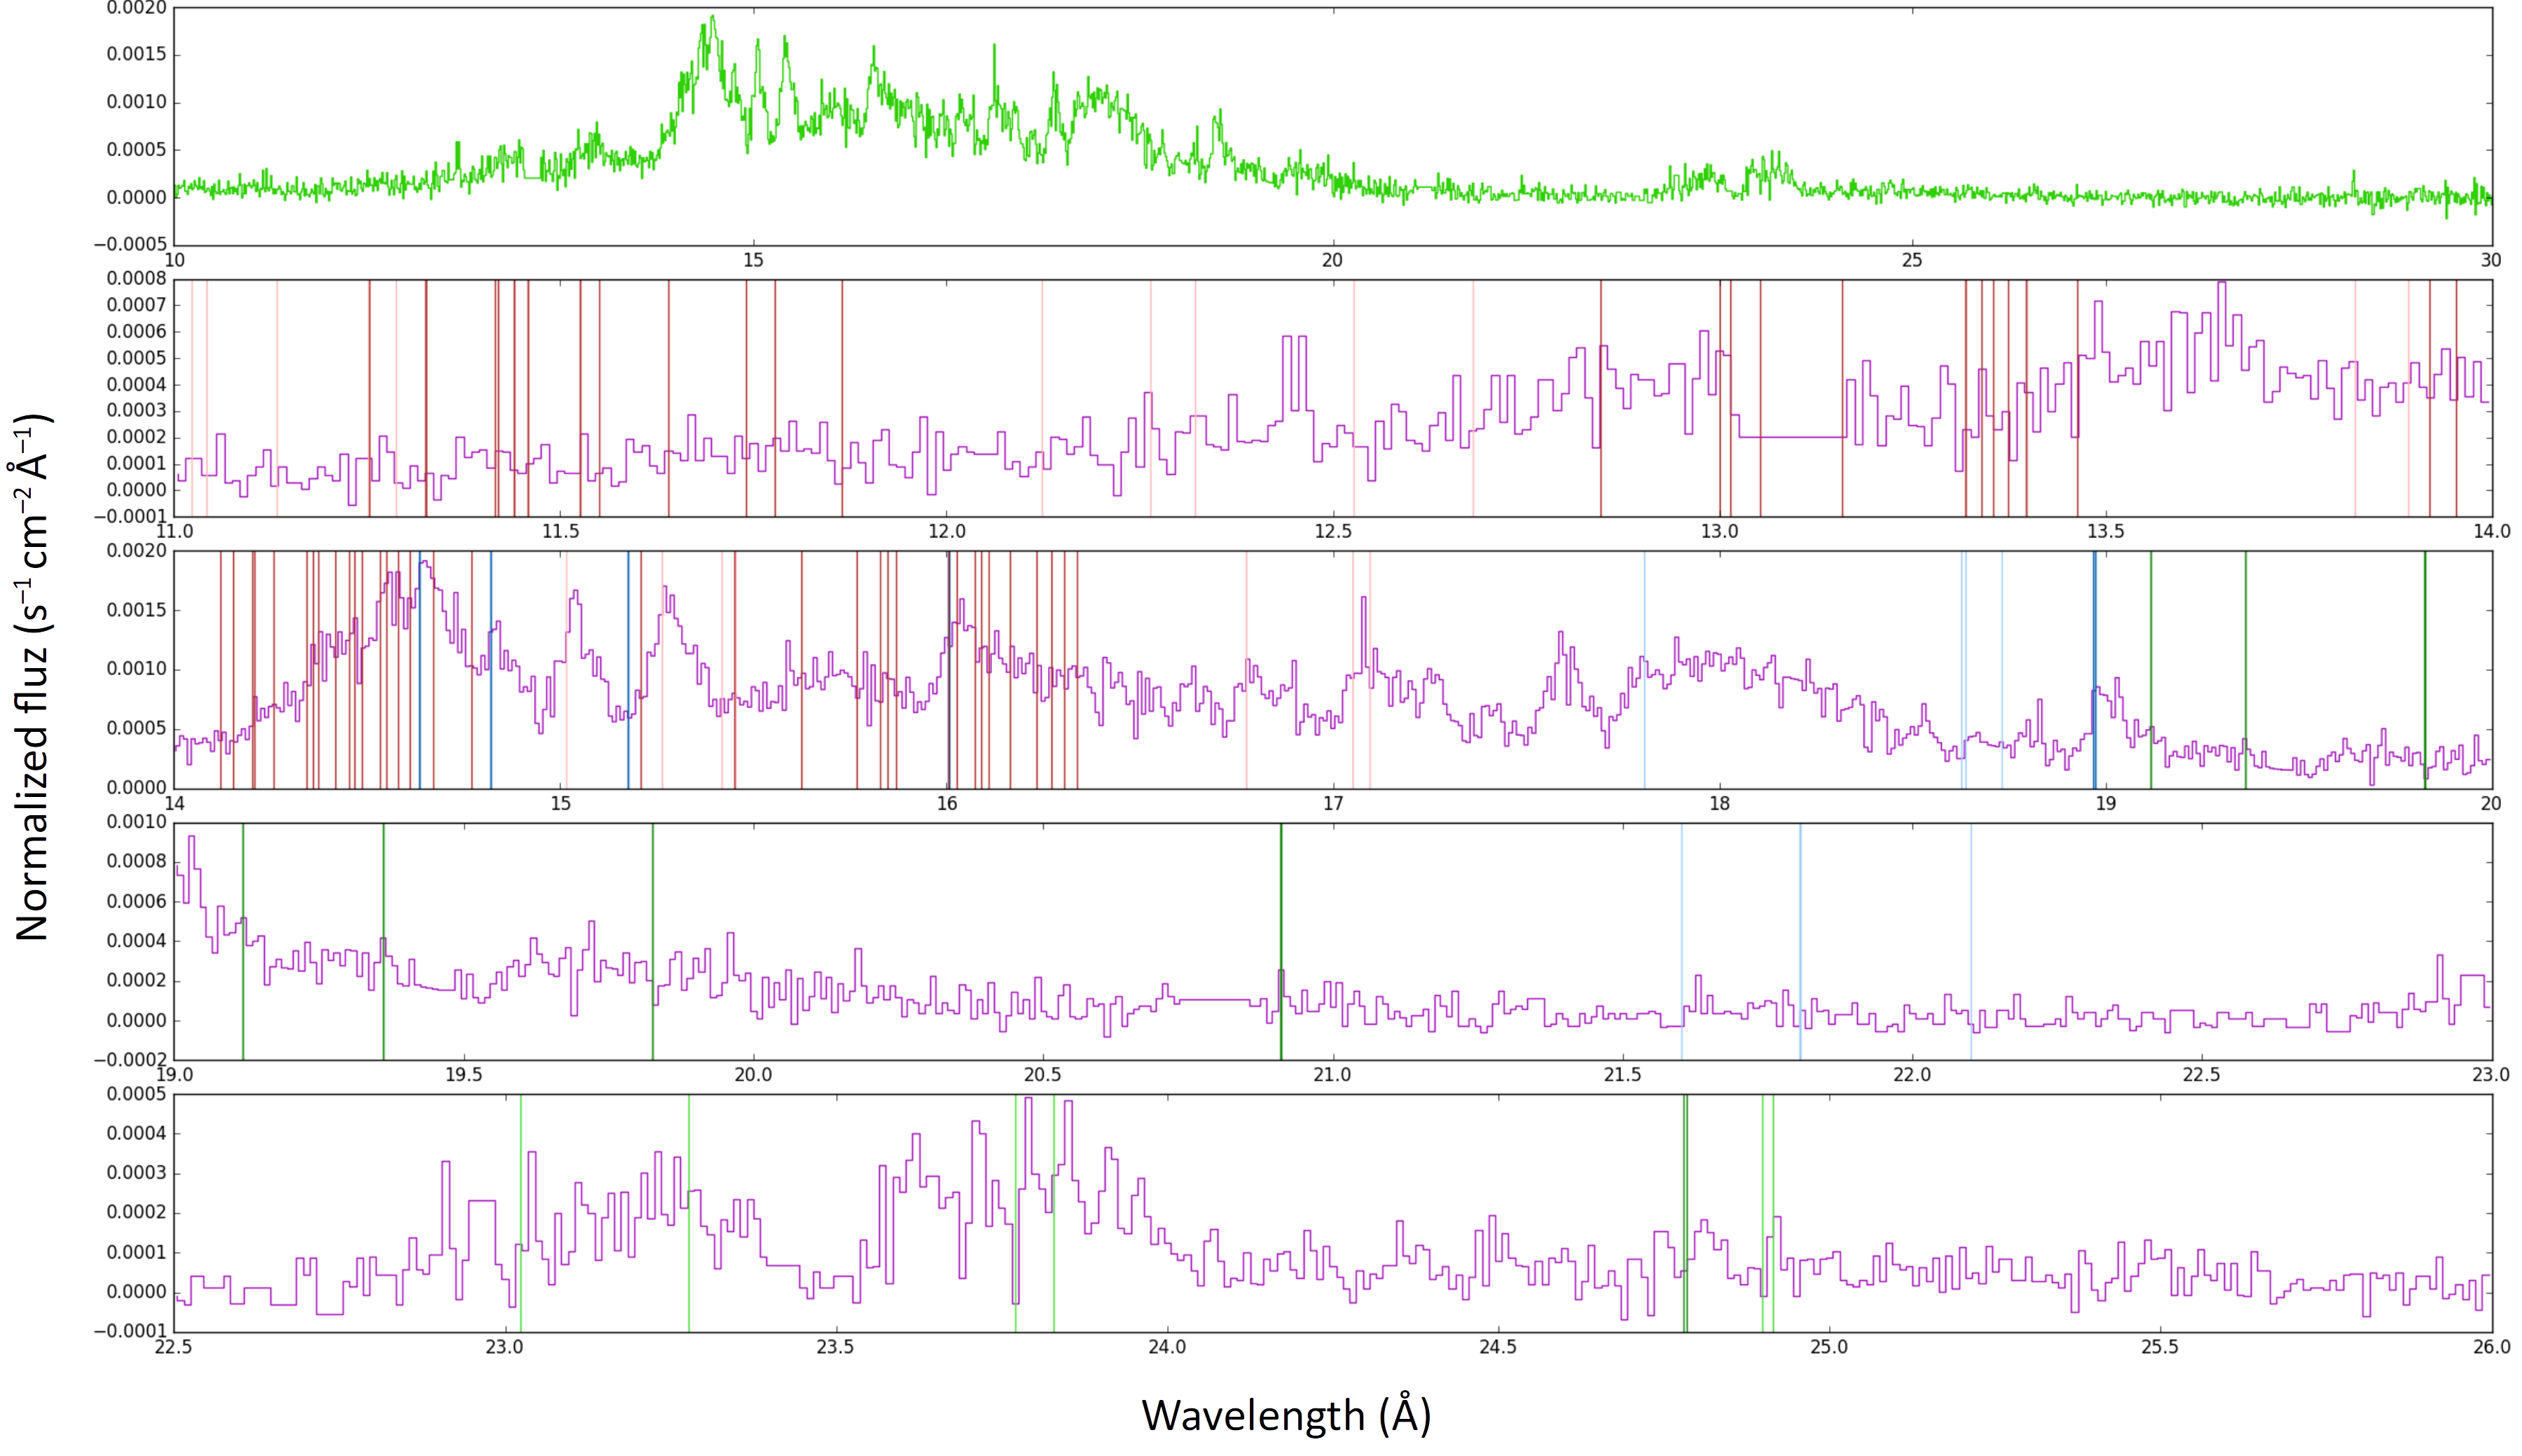
\includegraphics[width=\textwidth]{images/fig-line_identification-rgs.png}
		    	\caption{Overlay of transition lines on the fluxed RGS spectrum of \source\ for Obs. ID 0111150101}
		    	\label{fig:rgs-line-overlay}  
		    \end{figure}
		    
		    Absorption lines in the spectrum of \source\ arise due to the interaction of the emitted radiation with material along the line of sight. These lines exhibit diverse profiles, including shapes, widths, and shifts, which reflect the physical properties and dynamics of the absorbing material. Each absorption line corresponds to a specific transition of an atom or ion in the intervening material. Some of such lines are overlaid on the fluxed RGS spectrum of \source\ for the observation ID 0111150101, as presented in figure \ref{fig:rgs-line-overlay} \cite{bhattacharya2020python}. Here, the colour scheme is: N VI and N VII lines in light and dark green respectively, O VII and O VIII lines in light and dark blue respectively, Fe XVII and Fe XVIII lines in light and dark red respectively.
		    
		    By identifying the atomic species and transitions associated with each absorption feature, one can gain insight into the composition and kinematics of the absorbing medium. While optical spectra have been extensively studied by categorizing them based on the presence or absence of certain spectral lines and identifying anomalies such as unusually strong or weak lines, similar approaches have been challenging to apply to X-ray spectra due to their limited spectral resolution. However, with nearly two decades of high-resolution grating spectra available from X-ray observations, it is now opportune to explore and develop methods that leverage these data to categorize and analyze X-ray spectra in more nuanced ways, such as that by Ness et al. (2013) \cite{ness2013obscuration}.
    	
    	\subsection{Relative Strengths of Absorption Edges} \label{multi-obs:discussion:abs-edge-strength}
    		Absorption edges are included in an XSPEC model using the multiplicative component named \texttt{edge}. On a continuum model, an absorption edge may be modelled as follows:
		    \begin{align}
		    	M(E)=\begin{cases}
		    		{1;\quad E\leqslant E_\text{th}} \\
		    		{\exp{\left[ -D\left(\dfrac{E}{E_\text{th}}\right)^{-3} \right]};\quad E> E_\text{th}}
		    	\end{cases} \label{eqn:edge-comp}
		    \end{align}
		    In equation (\ref{eqn:edge-comp}), $E_\text{th}$ is the \textit{threshold energy} and $D$ is the \textit{absorption depth}. The model component is implemented with these two quantities being its parameters. The relative values of the absorption depths enables a comparison of the strengths of the absorption edges.
		    
		    The absorption depths calculated from the unfolded spectra, after obtaining the best fit to the model, are presented in table \ref{tab:abs-depth}. In all six observations, the same absorption edges were identified. For the observations made by ASCA, Chandra and XMM-Newton, the identified edges show the same trend with respect to the relative strengths of the absorption depths of these edges, i.e. the N $K$ absorption edge is the strongest, followed by the O $K$ edge, the Fe $L_3$ edge and the Ne $K$ edge with similar strengths.
		    
		    However, this is not the case for the three NICER observations, each of which show different edges to be the strongest. The reasons for such an inconsistency might range from instrumental effects (such as variations in the detector response with time, or changes in the gain calibration between observations) to issues with data reduction (such as inconsistencies in background subtraction, or inaccuracies in deadtime correction). Because NICER is a relatively new mission, it is a worthwhile exercise to investigate this particular inconsistency in absorption depth strength, which would include a detailed review of the NICER calibration documents, analysis of data from different detector regions, comparison with published data on similar sources and submission of relevant science proposals for new observations.